\documentclass{article}%
\usepackage[T1]{fontenc}%
\usepackage[utf8]{inputenc}%
\usepackage{lmodern}%
\usepackage{textcomp}%
\usepackage{lastpage}%
\usepackage{authblk}%
\usepackage{graphicx}%
%
\title{Mutation of the Diamond{-}Blackfan Anemia Gene Rps7 in Mouse Results in Morphological and Neuroanatomical Phenotypes}%
\author{Daniel Fernandez MD}%
\affil{Advanced Laboratory for Plant Genetic Engineering, Advanced Technology Development Centre, Indian Institute of Technology Kharagpur, Kharagpur, India}%
\date{01{-}01{-}2013}%
%
\begin{document}%
\normalsize%
\maketitle%
\section{Abstract}%
\label{sec:Abstract}%
A new patent with a major impact on the field of cell biology, advanced cancer research and cancer therapy.\newline%
Chronic Morphine Treatment Attenuates Cell Growth of Human BT474 Breast Cancer Cells by Rearrangement of the ErbB Signaling Network.\newline%
Chronic Morphine Treatment Attenuates Cell Growth of Human BT474 Breast Cancer Cells by Rearrangement of the ErbB Signaling Network.\newline%
Not only is this great new breakthrough to cancer research, it is also an important step forward in standard of care for human patients.\newline%
Circumcision removes more than one third of ovarian tumors in women, according to this Scientific American article. Now, we may be able to do the same for cancer.\newline%
People suffering from cancer are relatively isolated in their medical decisions; any decision in cancer treatment could have wide community implications. This new patent is based on the idea that a cell would develop a tumor by growing up, to far greater size than usual, by docking itself to a molecule on the cell membrane, or outside its own genome. This mechanism allows for simultaneous localization and localization to make sure that tumor cells develop in sequence and proportion to each other, while also extending the range of activation activities of the targeted genes, known as metamorous contracting, or MET. Thus, this could be the basis for a new type of chronic chemotherapy, or to increase the intensity and duration of chemotherapeutic treatment for more patients. This invention could also play a role in identifying weak and persistent tumor stem cells or other types of tumors to expand and promote cell growth as an alternative in disease treatment.\newline%
Ann Marie Kazakoff\newline%
President of the Journal of Molecular and Cellular oncology\newline%
{[}email protected{]}

%
\subsection{Image Analysis}%
\label{subsec:ImageAnalysis}%


\begin{figure}[h!]%
\centering%
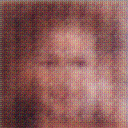
\includegraphics[width=150px]{500_fake_images/samples_5_291.png}%
\caption{A Black And White Photo Of A Black And White Photo}%
\end{figure}

%
\end{document}